\documentclass[]{article}

% Imported Packages
%------------------------------------------------------------------------------
\usepackage{amssymb}
\usepackage{amstext}
\usepackage{amsthm}
\usepackage{amsmath}
\usepackage{enumerate}
\usepackage{fancyhdr}
\usepackage[margin=1in]{geometry}
\usepackage{graphicx}
%\usepackage{extarrows}
%\usepackage{setspace}
%------------------------------------------------------------------------------

% Header and Footer
%------------------------------------------------------------------------------
\pagestyle{plain}  
\renewcommand\headrulewidth{0.4pt}                                      
\renewcommand\footrulewidth{0.4pt}                                    
%------------------------------------------------------------------------------

% Title Details
%------------------------------------------------------------------------------
\title{Deliverable \#2}
\author{SE 3A04: Software Design II -- Large System Design}
\date{}                               
%------------------------------------------------------------------------------

% Document
%------------------------------------------------------------------------------
\begin{document}

\maketitle	
\noindent{\bf Tutorial Number:} T03\\
{\bf Group Number:} G8 \\
{\bf Group Members:} 
\begin{itemize}
	\item Hashim Bukhtiar
	\item Jaden Moore
	\item James Ariache
	\item Olivia Reich
	\item Omar Abdelhamid
\end{itemize}

\section*{IMPORTANT NOTES}
\begin{itemize}
	%	\item You do \underline{NOT} need to provide a text explanation of each diagram; the diagram should speak for itself
	\item Please document any non-standard notations that you may have used
	\begin{itemize}
		\item \emph{Rule of Thumb}: if you feel there is any doubt surrounding the meaning of your notations, document them
	\end{itemize}
	\item Some diagrams may be difficult to fit into one page
	\begin{itemize}
		\item Ensure that the text is readable when printed, or when viewed at 100\% on a regular laptop-sized screen.
		\item If you need to break a diagram onto multiple pages, please adopt a system of doing so and thoroughly explain how it can be reconnected from one page to the next; if you are unsure about this, please ask about it
	\end{itemize}
	\item Please submit the latest version of Deliverable 1 with Deliverable 2
	\begin{itemize}
		\item Indicate any changes you made.
	\end{itemize}
	\item If you do \underline{NOT} have a Division of Labour sheet, your deliverable will \underline{NOT} be marked
\end{itemize}

\newpage
\section{Introduction}
\label{sec:introduction}
% Begin Section

\subsection{Purpose}
\label{sub:purpose}
% Begin SubSection
This document provides a high-level overview of the RideRecon car identification system architecture, including high-level design considerations of the system and design consideration for various subsystems. This document is intended for internal RideRecon stakeholders, including but not limited to, project managers, developers, domain experts, and RideRecon team members/investors. \\

\noindent Note that RideRecon Deliverable 1 should be read before Deliverable 2, and technical knowledge may be beneficial in better understanding this document's contents.

% End SubSection

\subsection{System Description}
\label{sub:system_description}
% Begin SubSection
The RideRecon system is designed to identify vehicles based on both text and image inputs, leveraging multiple expert modules (such as a reverse image search engine, a text-based LLM, and trained ML models). To integrate these diverse experts effectively, RideRecon follows a blackboard architecture. In this approach, all relevant data—user inputs, partial identifications, and expert findings—are posted to a central “blackboard.” Each expert module reads from this shared repository, processes the data according to its specialization, and writes back its results. This iterative process continues until a consensus or a conflict resolution mechanism determines the final identification outcome.\\

\noindent A blackboard architecture is well-suited to RideRecon because it supports concurrent data processing among the different expert modules, each of which may require varying amounts of time or resources. It also simplifies the system’s ability to integrate new expert modules in the future—such as additional AI models or external APIs—by giving them the same shared data repository to read from and write to. This design ensures that updates or new insights posted by one expert can immediately inform the decision-making of others, resulting in a flexible, extensible platform for complex vehicle identification tasks.

% End SubSection

\subsection{Overview}
\label{sub:overview}
% Begin SubSection
Describe what the rest of the document contains and explain how the document is organised (e.g. "In Section 2 we discuss...in Section 3...").

% End SubSection

% End Section

\section{Analysis Class Diagram}
\label{sec:analysis_class_diagram}
% Begin Section
\begin{center}
	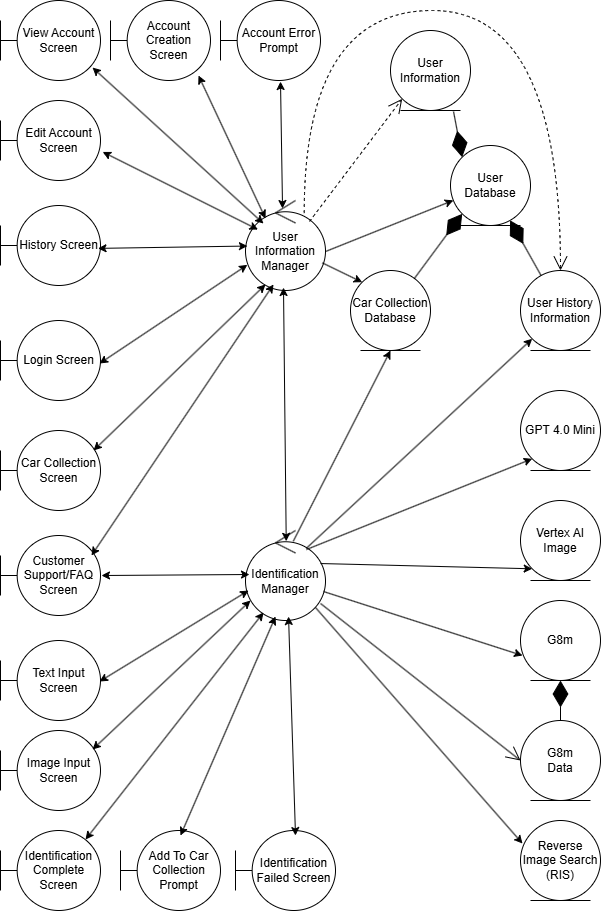
\includegraphics[scale=0.5]{images/AnalysisDiagram_compacted.png}\\
	\textbf{Figure 1.} Analysis class diagram for the RideRecon system, showing interactions between user interface screens, core system managers, databases, and expert modules for user management and vehicle identification.
\end{center}
% End Section


\section{Architectural Design}
\label{sec:architectural_design}
% Begin Section
This section should provide an overview of the overall architectural design of your application. Your overall architecture should show the division of the system into subsystems with high cohesion and low coupling.

\subsection{System Architecture}
\label{sub:system_architecture}
% Begin SubSection
\begin{itemize}
	\item Identify and explain the overall architecture of your system
	\item Be sure to clearly state the name of the architecture you used (this is the name of the architectural pattern, not the name of your system)
	\item Provide the reasoning and justification of the choice of architecture
	\item Provide a structural architecture diagram showing the relationship among the subsystems (if appropriate)
	\item List any design alternatives you considered, but eliminated (and explain why you eliminated them)
\end{itemize}
% End SubSection

\subsection{Subsystems}
\label{sub:subsystems}
% Begin SubSection
The RideRecon system is divided into several key subsystems, each with a distinct role that contributes to the overall vehicle identification process. At its core, RideRecon employs a hybrid architecture that combines a blackboard approach—enabling multiple expert modules to collaboratively process inputs—with a repository-style design that robustly manages and stores data. This design not only ensures accurate vehicle identification but also supports continuous improvement through systematic data management.\\

\noindent The Input Management Subsystem is responsible for capturing and preprocessing user inputs, including both text and image data. It ensures that all input data is correctly formatted and validated before being fed into the core processing units. The Identification Subsystem acts as the central processing hub where diverse expert modules—such as the Vertex AI Image Model, Reverse Image Search, a specialized text-based LLM, and an internally trained ML model—post their analyses to a shared blackboard, collaboratively resolving any conflicts to produce a final identification. The Data Management Subsystem leverages repository principles to securely store both raw user inputs and processed outputs, which supports future retraining, auditing, and model improvement. Finally, the Account Management Subsystem handles user authentication and profile management, ensuring personalized interactions and maintaining a comprehensive record of user engagements. Together, these interconnected subsystems create a robust and scalable platform tailored to the challenges of dynamic, real-world vehicle identification.

% End SubSection

% End Section
	
\section{Class Responsibility Collaboration (CRC) Cards}
\label{sec:class_responsibility_collaboration_crc_cards}
% Begin Section
This section should contain all of your CRC cards.

\begin{itemize}
	\item Provide a CRC Card for each identified class
	\item Please use the format outlined in tutorial, i.e., 
	\begin{table}[ht]
		\centering
		\begin{tabular}{|p{5cm}|p{5cm}|}
		\hline 
		 \multicolumn{2}{|l|}{\textbf{Class Name:}} \\
		\hline
		\textbf{Responsibility:} & \textbf{Collaborators:} \\
		\hline
		\vspace{1in} & \\
		\hline
		\end{tabular}
	\end{table}
	
\end{itemize}
% End Section

\appendix
\section{Division of Labour}
\label{sec:division_of_labour}
% Begin Section
Include a Division of Labour sheet which indicates the contributions of each team member. This sheet must be signed by all team members.
% End Section
\begin{table}[h!]
\centering
\begin{tabular}{|p{3cm}|p{3.5cm}|p{3cm}|p{3cm}|p{3.5cm}|}
\hline
Hashim Bukhtiar & Jaden Moore & James Ariache & Olivia Reich & Omar Abdelhamid \\ \hline
1.1, 1.2, 3.2 & X Cards in Section 4 & Section 2 & Section 3.1 & Y Cards in Section 4 \\ 
Compiled Final Doc &  &  &  & Section 1.3 \\
\includegraphics[height=1cm]{../D1/images/hashim_signature.png} & \includegraphics[height=1cm]{../D1/images/Jaden_signature.jpg} &
\includegraphics[scale=0.1]{../D1/images/james_signature.png}& \includegraphics[height=0.6cm]{../D1/images/olivia_signature.png} & \includegraphics[height=0.6cm]{../D1/images/omar_signature.png}  \\
\hline
\end{tabular}
\caption{Division of Labour} 
\label{tab:division_of_labour}
\end{table}

\end{document}
%------------------------------------------------------------------------------